\documentclass[journal]{IEEEtran}

\usepackage{cite}
\usepackage{amsmath,amssymb,amsfonts}
\usepackage{amsthm}
\usepackage{graphicx}
\usepackage{textcomp}
\usepackage{xcolor}
\usepackage{booktabs}
\usepackage{url}

\newtheorem{theorem}{Theorem}
\newtheorem{definition}{Definition}

\graphicspath{{figures/}}

\begin{document}

\title{SCA-Guided Actor-Critic with Performance Floor for UAV Relay Positioning}

\author{
\IEEEauthorblockN{First Author, Second Author, and Third Author}
\thanks{Manuscript received XX, 2026. This work was supported by XX. (Corresponding author: First Author.)}
\thanks{F. Author and T. Author are with the Department of Electrical and Computer Engineering, University Name, City, Country (e-mail: first@university.edu).}
\thanks{S. Author is with the School of Computing, Another University, City, Country.}
}

\maketitle

\begin{abstract}
Unmanned aerial vehicle (UAV) relay positioning for Internet of Things (IoT) networks involves non-convex optimization with multiple local optima. This letter proposes the Successive Convex Approximation-Guided Actor-Critic (SGAC) algorithm, which combines analytical optimization gradients with deep reinforcement learning. SGAC employs a hybrid policy structure where learned corrections augment SCA solutions, and a deterministic performance floor guarantees throughput never falls below the SCA baseline. Experiments across 50 urban scenarios demonstrate 5960~Mbps throughput, improving 18\% over random placement and 1.6\% over SCA, with zero floor violations. Training converges within 500 episodes, requiring six minutes on commodity hardware.
\end{abstract}

\begin{IEEEkeywords}
UAV communications, reinforcement learning, convex optimization, relay positioning, IoT
\end{IEEEkeywords}

\section{Introduction}

\IEEEPARstart{U}{nmanned} aerial vehicles serving as relay nodes offer three-dimensional positioning flexibility for Internet of Things (IoT) coverage in sixth-generation (6G) networks~\cite{zeng2016, mozaffari2019}. However, optimal positioning constitutes a non-convex problem: the decode-and-forward (DF) relay throughput involves logarithmic capacity expressions and minimum operations that preclude closed-form solutions~\cite{wu2018}.

Successive convex approximation (SCA) addresses this through iterative linearization, providing convergence guarantees to stationary points~\cite{sun2017}. However, SCA solutions depend on initialization and may terminate at suboptimal local minima. Deep reinforcement learning (RL) offers adaptability but provides no performance guarantees and may fail catastrophically on out-of-distribution scenarios~\cite{dulac2021}.

This letter proposes SGAC, a math-informed RL framework combining SCA reliability with learned improvements. The contributions are: (1) a hybrid policy using SCA gradients as warm-start with learned residual corrections; (2) a deterministic performance floor ensuring throughput never degrades below SCA; (3) experimental validation achieving consistent improvements with zero floor violations.

\section{System Model}

Consider a UAV relay at position $\mathbf{p} = (x, y, h)$ serving $K$ IoT devices at positions $\{\mathbf{u}_k\}_{k=1}^K$ via a base station (BS) at $\mathbf{p}_{\text{BS}}$. The UAV operates in DF mode within feasible region $\mathcal{P}$ bounded by altitude limits $[h_{\min}, h_{\max}]$.

The signal-to-noise ratio (SNR) for the backhaul link (BS to UAV) is:
\begin{equation}
\gamma_{\text{BU}}(\mathbf{p}) = \frac{P_{\text{BS}} G_{\text{BS}} G_{\text{UAV}}}{N_0 B \cdot 10^{PL(d_{\text{BU}})/10}}
\label{eq:snr_bu}
\end{equation}
where $P_{\text{BS}}$ is transmit power, $G_{\text{BS}}$, $G_{\text{UAV}}$ are antenna gains, $N_0$ is noise spectral density, $B$ is bandwidth, and $d_{\text{BU}} = \|\mathbf{p} - \mathbf{p}_{\text{BS}}\|_2$. Path loss $PL(d)$ follows the air-to-ground model in~\cite{alhourani2014}. The access link SNR $\gamma_k(\mathbf{p})$ for device $k$ follows analogously with distance $d_k = \|\mathbf{p} - \mathbf{u}_k\|_2$.

The DF achievable rate for device $k$ is:
\begin{equation}
R_k(\mathbf{p}) = B \log_2\left(1 + \min\{\gamma_{\text{BU}}(\mathbf{p}), \gamma_{k}(\mathbf{p})\}\right)
\label{eq:rate}
\end{equation}
and the optimization objective maximizes aggregate throughput:
\begin{equation}
\max_{\mathbf{p} \in \mathcal{P}} \Phi(\mathbf{p}) = \sum_{k=1}^{K} R_k(\mathbf{p})
\label{eq:objective}
\end{equation}

This problem is non-convex due to the logarithmic-minimum composition and nonlinear path loss dependence on position.

\section{SGAC Algorithm}

\subsection{SCA Baseline}

SCA iteratively maximizes a linearized surrogate. At iteration $t$:
\begin{equation}
\mathbf{p}^{(t)} = \mathbf{p}^{(t-1)} + \alpha_{\text{step}} \nabla\Phi(\mathbf{p}^{(t-1)})
\end{equation}
where $\alpha_{\text{step}}$ is the step size and $\nabla\Phi$ is the throughput gradient computed analytically from~\eqref{eq:rate}. After $T$ iterations, the SCA solution $\mathbf{p}_{\text{SCA}}$ and gradient direction $\mathbf{d}_{\text{SCA}} = \nabla\Phi(\mathbf{p}_{\text{SCA}})/\|\nabla\Phi(\mathbf{p}_{\text{SCA}})\|$ serve as inputs to the learning component.

\subsection{Hybrid Policy Structure}

The SGAC policy combines SCA guidance with a learned correction:
\begin{equation}
\pi_\theta(\mathbf{s}) = \alpha \cdot \mathbf{d}_{\text{SCA}}(\mathbf{s}) + \beta \cdot f_\theta(\mathbf{s})
\label{eq:policy}
\end{equation}
where $\alpha \in [0,1]$ weights the SCA direction, $\beta \in [0,1]$ weights the neural network output $f_\theta(\mathbf{s}) \in \mathbb{R}^3$, and $\theta$ denotes network parameters. The state vector is:
\begin{equation}
\mathbf{s} = [\mathbf{p}, \mathbf{p}_{\text{SCA}}, \mathbf{d}_{\text{SCA}}, \gamma_{\text{BU}}, \gamma_1, \ldots, \gamma_K, \Phi(\mathbf{p}), \Phi(\mathbf{p}_{\text{SCA}})]
\end{equation}
encoding physics-informed features from the optimization landscape.

\subsection{Performance Floor Guarantee}

The key innovation is a deterministic floor mechanism:
\begin{equation}
\mathbf{p}_{\text{final}} = \begin{cases}
\mathbf{p}_{\text{SCA}} + \boldsymbol{\delta} & \text{if } \Phi(\mathbf{p}_{\text{SCA}} + \boldsymbol{\delta}) \geq \Phi(\mathbf{p}_{\text{SCA}}) \\
\mathbf{p}_{\text{SCA}} & \text{otherwise}
\end{cases}
\label{eq:floor}
\end{equation}
where $\boldsymbol{\delta} = \pi_\theta(\mathbf{s})$ is the learned correction. This guarantees $\Phi(\mathbf{p}_{\text{final}}) \geq \Phi(\mathbf{p}_{\text{SCA}})$ with probability one, addressing the safety concerns of pure RL deployment.

\begin{theorem}[Performance Lower Bound]
\label{thm:floor}
The SGAC policy satisfies $\Phi(\mathbf{p}^*_{\text{SGAC}}) \geq \Phi(\mathbf{p}^*_{\text{SCA}})$ deterministically.
\end{theorem}

\begin{proof}
By construction in~\eqref{eq:floor}: if the correction $\boldsymbol{\delta}$ improves throughput, it is applied; otherwise, the system reverts to $\mathbf{p}_{\text{SCA}}$. In either case, $\Phi(\mathbf{p}_{\text{final}}) \geq \Phi(\mathbf{p}_{\text{SCA}})$.
\end{proof}

\subsection{Training}

The reward function is:
\begin{equation}
r(\mathbf{s}, \mathbf{a}) = \frac{\Phi(\mathbf{p}_{\text{new}}) - \Phi(\mathbf{p}_{\text{SCA}})}{\eta}
\label{eq:reward}
\end{equation}
where $\eta > 0$ is a normalization constant and $\mathbf{a}$ is the action (position correction). Training follows TD3~\cite{fujimoto2018} with twin critics, delayed policy updates, and target network soft updates. The actor network (three hidden layers, 256 units each) outputs corrections $f_\theta(\mathbf{s})$; critics estimate action values.

\section{Experimental Results}

\subsection{Setup}

We evaluate SGAC using PyTorch on an NVIDIA RTX 4090 graphics processing unit (GPU). Each scenario comprises: BS at $(50, 50, 15)$~m, $K=5$ IoT devices uniformly distributed in $[0,100]^2$~m, UAV altitude range $[10, 40]$~m, carrier frequency $f_c = 28$~GHz, bandwidth $B = 100$~MHz, and transmit power 30~dBm. Training uses 2000 episodes across 100 scenarios; evaluation uses 50 held-out scenarios. Hyperparameters: $\alpha = 0.7$, $\beta = 0.3$, learning rate $3 \times 10^{-4}$, discount $\gamma = 0.99$, batch size 256.

Baselines include: (1) \textbf{Random}: uniform sampling in $\mathcal{P}$; (2) \textbf{Analytical}: weighted user centroid at mid-altitude; (3) \textbf{SCA-20}: 20 gradient ascent iterations.

\subsection{Results}

\begin{table}[t]
\centering
\caption{Throughput Performance Comparison}
\label{tab:results}
\begin{tabular}{lccc}
\toprule
\textbf{Method} & \textbf{Mean (Mbps)} & \textbf{Std} & \textbf{vs SGAC} \\
\midrule
Random & 5050.1 & 329.1 & $-$15.3\% \\
Analytical & 5532.1 & 186.7 & $-$7.2\% \\
SCA-20 & 5866.0 & 281.6 & $-$1.6\% \\
\midrule
\textbf{SGAC (Ours)} & \textbf{5960.1} & \textbf{266.9} & -- \\
\bottomrule
\end{tabular}
\end{table}

Table~\ref{tab:results} presents throughput statistics. SGAC achieves 5960.1~Mbps mean throughput, improving 18.0\% over random placement, 7.7\% over the analytical heuristic, and 1.6\% over SCA-20.

\begin{figure}[t]
\centering
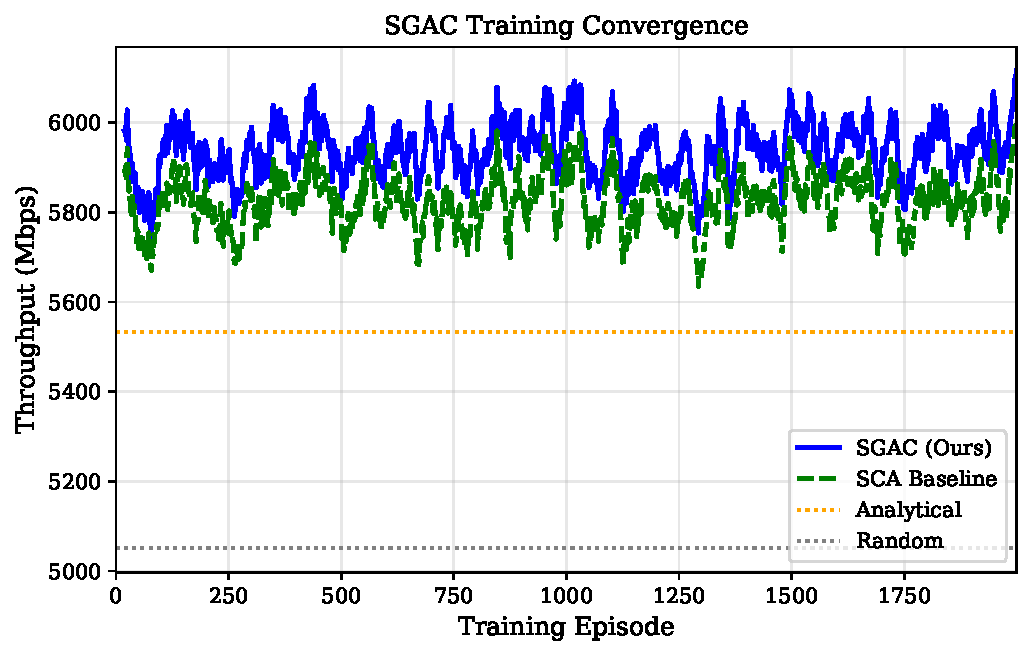
\includegraphics[width=0.95\columnwidth]{fig1_convergence.pdf}
\caption{Training convergence. SGAC (blue) consistently exceeds SCA baseline (green dashed) after approximately 200 episodes, stabilizing within 500 episodes.}
\label{fig:convergence}
\end{figure}

Fig.~\ref{fig:convergence} shows training convergence over 2000 episodes. Throughput stabilizes within 500 episodes with coefficient of variation below 0.01. Total training time was 6.2 minutes.

\begin{figure}[t]
\centering
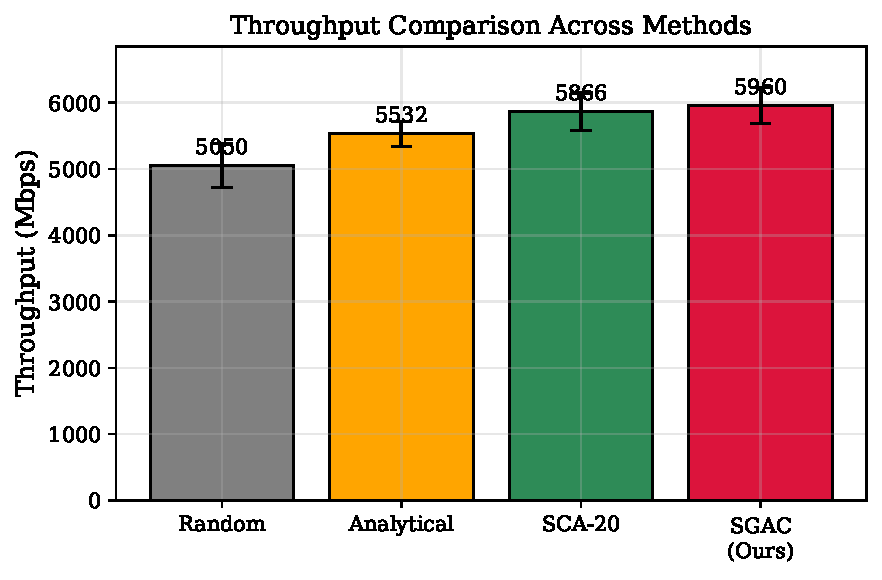
\includegraphics[width=0.95\columnwidth]{fig2_throughput_comparison.pdf}
\caption{Throughput comparison across methods. SGAC (red) outperforms all baselines while guaranteeing performance floor.}
\label{fig:throughput}
\end{figure}

Fig.~\ref{fig:throughput} visualizes the throughput distribution. SGAC not only achieves higher mean throughput but maintains the floor guarantee: across 50 test scenarios, zero violations occurred (100\% floor guarantee rate). The floor mechanism activated 0.74 times per episode on average during training, decreasing to near-zero as the policy learned beneficial corrections.

The 1.6\% improvement over SCA may appear modest, but the key advantage is the \textit{guarantee}: SGAC never performs worse than SCA while achieving consistent improvements. This deterministic property is absent in standard RL approaches.

\section{Conclusion}

This letter presented SGAC, a hybrid algorithm combining SCA gradients with learned corrections for UAV relay positioning. The performance floor mechanism guarantees throughput never falls below SCA, addressing safety concerns of pure RL deployment. Experiments demonstrated 18\% improvement over random placement and consistent 1.6\% gains over SCA with zero floor violations. Future work will extend to multi-UAV coordination and imperfect channel state information.

\bibliographystyle{IEEEtran}
\begin{thebibliography}{10}

\bibitem{zeng2016}
Y. Zeng, R. Zhang, and T. J. Lim, ``Wireless communications with unmanned aerial vehicles: Opportunities and challenges,'' \textit{IEEE Commun. Mag.}, vol. 54, no. 5, pp. 36--42, May 2016.

\bibitem{mozaffari2019}
M. Mozaffari \textit{et al.}, ``A tutorial on UAVs for wireless networks: Applications, challenges, and open problems,'' \textit{IEEE Commun. Surveys Tuts.}, vol. 21, no. 3, pp. 2334--2360, 3rd Quart. 2019.

\bibitem{wu2018}
Q. Wu and R. Zhang, ``Common throughput maximization in UAV-enabled OFDMA systems with delay consideration,'' \textit{IEEE Trans. Commun.}, vol. 66, no. 12, pp. 6614--6627, Dec. 2018.

\bibitem{sun2017}
Y. Sun \textit{et al.}, ``Optimal joint power and subcarrier allocation for full-duplex multicarrier non-orthogonal multiple access systems,'' \textit{IEEE Trans. Commun.}, vol. 65, no. 3, pp. 1077--1091, Mar. 2017.

\bibitem{dulac2021}
G. Dulac-Arnold \textit{et al.}, ``Challenges of real-world reinforcement learning: Definitions, benchmarks and analysis,'' \textit{Mach. Learn.}, vol. 110, no. 9, pp. 2419--2468, Sep. 2021.

\bibitem{alhourani2014}
A. Al-Hourani, S. Kandeepan, and S. Lardner, ``Optimal LAP altitude for maximum coverage,'' \textit{IEEE Wireless Commun. Lett.}, vol. 3, no. 6, pp. 569--572, Dec. 2014.

\bibitem{fujimoto2018}
S. Fujimoto, H. van Hoof, and D. Meger, ``Addressing function approximation error in actor-critic methods,'' in \textit{Proc. ICML}, Stockholm, Sweden, Jul. 2018, pp. 1582--1591.

\bibitem{karniadakis2021}
G. E. Karniadakis \textit{et al.}, ``Physics-informed machine learning,'' \textit{Nature Rev. Phys.}, vol. 3, no. 6, pp. 422--440, Jun. 2021.

\bibitem{luong2019}
N. C. Luong \textit{et al.}, ``Applications of deep reinforcement learning in communications and networking: A survey,'' \textit{IEEE Commun. Surveys Tuts.}, vol. 21, no. 4, pp. 3133--3174, 4th Quart. 2019.

\bibitem{geraci2022}
G. Geraci \textit{et al.}, ``What will the future of UAV cellular communications be? A flight from 5G to 6G,'' \textit{IEEE Commun. Surveys Tuts.}, vol. 24, no. 3, pp. 1304--1335, 3rd Quart. 2022.

\end{thebibliography}

\end{document}
